\documentclass[11pt, oneside]{article}   	% use "amsart" instead of "article" for AMSLaTeX format
\usepackage{geometry}                		% See geometry.pdf to learn the layout options. There are lots.
\geometry{letterpaper}                   		% ... or a4paper or a5paper or ... 
%\geometry{landscape}                		% Activate for rotated page geometry
%\usepackage[parfill]{parskip}    		% Activate to begin paragraphs with an empty line rather than an indent
\usepackage{graphicx}				% Use pdf, png, jpg, or eps§ with pdflatex; use eps in DVI mode
								% TeX will automatically convert eps --> pdf in pdflatex		
\usepackage{amssymb}
\usepackage{minted}

%SetFonts

%SetFonts


\title{Brief Article}
\author{The Author}
%\date{}							% Activate to display a given date or no date

\begin{document}
%\maketitle
%\section{}
%\subsection{}
\begin{flushright}
Donovan Guelde\\
CSCI 5352\\
PS3\\
\end{flushright}
1. $Q = \sum_r (e_{rr} -a_r^2)$ Eq. (7.76)\\
\indent $e_{rr}$ is given by the diagonals of the table given in Problem 1, since this value represents the fraction of all edges that connect like vertex to like vertex (in other words, a given edge $e$ that is included in a diagonal has one endpoint connected to a man of ethnicity $r$, and the other to a woman of ethnicity $r$).  $a_r$, the number of edges that connect to a given vertex type $r$, can be found by: $A_{rr} +\sum_{s \ne r} (A_{rs} + A_{sr})$.  This represents the number of edges with at least one endpoint connecting to vertex type $r$.\\\\
\indent This gives us the following values:
\begin{tabular}{|c|c|c|c|}
\hline
  Ethnicity $$& $e_{rr}$ & $a_r$&{${a_r}^2$}\\
  \hline
  Black & 0.258 & 0.352 & 0.124\\
  \hline
  Hispanic & 0.157&0.292&0.085\\
  \hline
  White & 0.306 & 0.494 & 0.244\\
  \hline
  Other & 0.016 & 0.119 & 0.014\\
 \hline
   \end{tabular}
 \\
 So, by Eq.(7.76), Q = 0.27\\
 \indent Overall, the community exhibits distinct homophily.  The only outlier is the $other$ vertex type, which is not surprising, considering that this vertex type is actually a collection of vertices of varying types.  These smaller subtypes may be small minorities of the community as a whole.\\
 \\
 2. a.  A line graph with n vertices (n-1 total edges, 2n-2 total endpoints), whose nodes  are divided into two contiguous groups, $r$ and $\lnot r$ results in the following configuration:\\
 \begin{tabular}{|c|c|c|}
 \hline
 Component & ($e_{rr})$ & ($a_r$)\\
 \hline
 $r$ & $\frac{r-1}{n-1}$ & $\frac{2r-1}{2n-2}$\\
 \hline
 $\lnot r$ & $\frac{n-r-1}{n-1}$ & $\frac{2n-2r-1}{2n-2}$\\
 \hline
\end{tabular}
\\\\
* $e_{rr}$ is the number of nodes that link vertices of the same component.  \\
$a_r$ is calculated by $\frac{number\ of\ endpoints\ attached\ to\ a\ component's\ vertices}{total\ number\ of\ endpoints\ in\ the\ graph}$\\
$Q = \sum_r (e_{rr} - {a_2}^2$)\\\\
$Q= \frac{r-1}{n-1} - (\frac{2r-1}{2n-2})^2 + \frac{n-r-1}{n-1} - (\frac{2n-2r-2}{2n-2})^2$\\\\
$Q=\frac{3-4n+4rn-4r^2}{2(n-1)^2}$\\\\\\
2. b.  If the graph has n nodes where n is even, then each component has $r = \lnot r = \frac{n}{2}$ nodes.  To maximize Q, we can use the first and second derivatives of the result from 2.a.\\
$\frac{d}{dr} \frac{3-4n+4rn-4r^2}{2(n-1)^2}= \frac{2(n-2r)}{(n-1)^2}$ which equals 0 at $r = \frac{n}{2}$, and
$\frac{d^2}{du^2} = \frac{-4}{(n-1)^2}$, which is negative for all values of r, so $r=\frac{n}{2}$ is a global maximum for the  equation $Q = \frac{3-4n+4rn-4r^2}{2(n-1)^2}$.  This tells us that, when n is even, the division resulting in optimal modularity is one where both components have an equal number of nodes.\\\\\\
3.  Using the greedy agglomerative algorithm on the Zachary Karate Club network, the maximum Q score achieved was 0.3806 with three groups (after 31 merges), as shown here:\\  
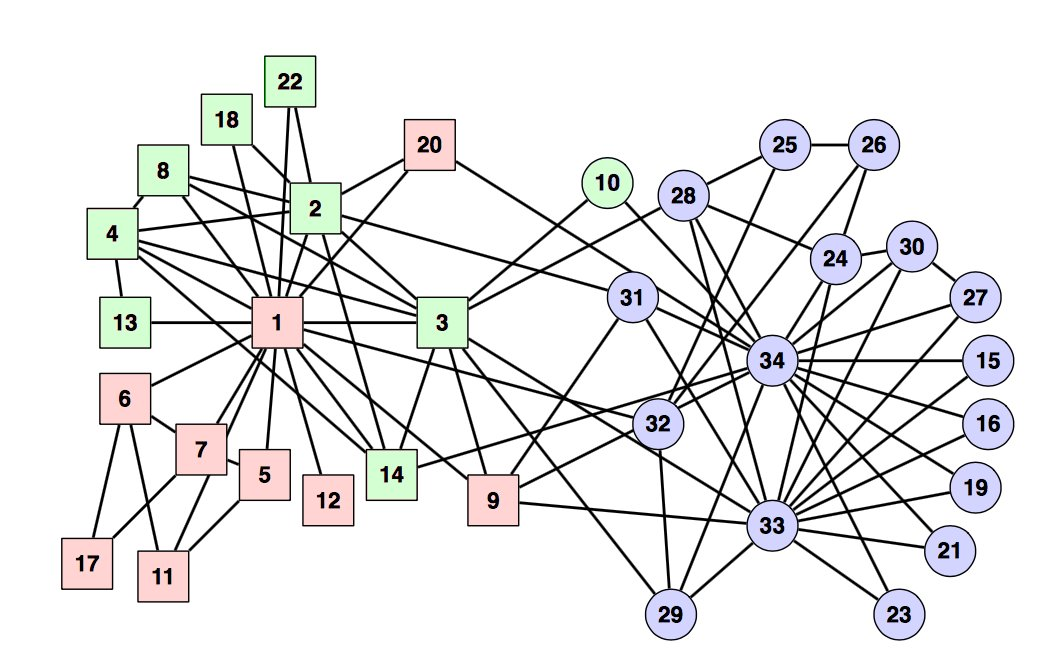
\includegraphics[scale=.25]{karate.jpg}\\
Q as a function of number of merges gives:\\
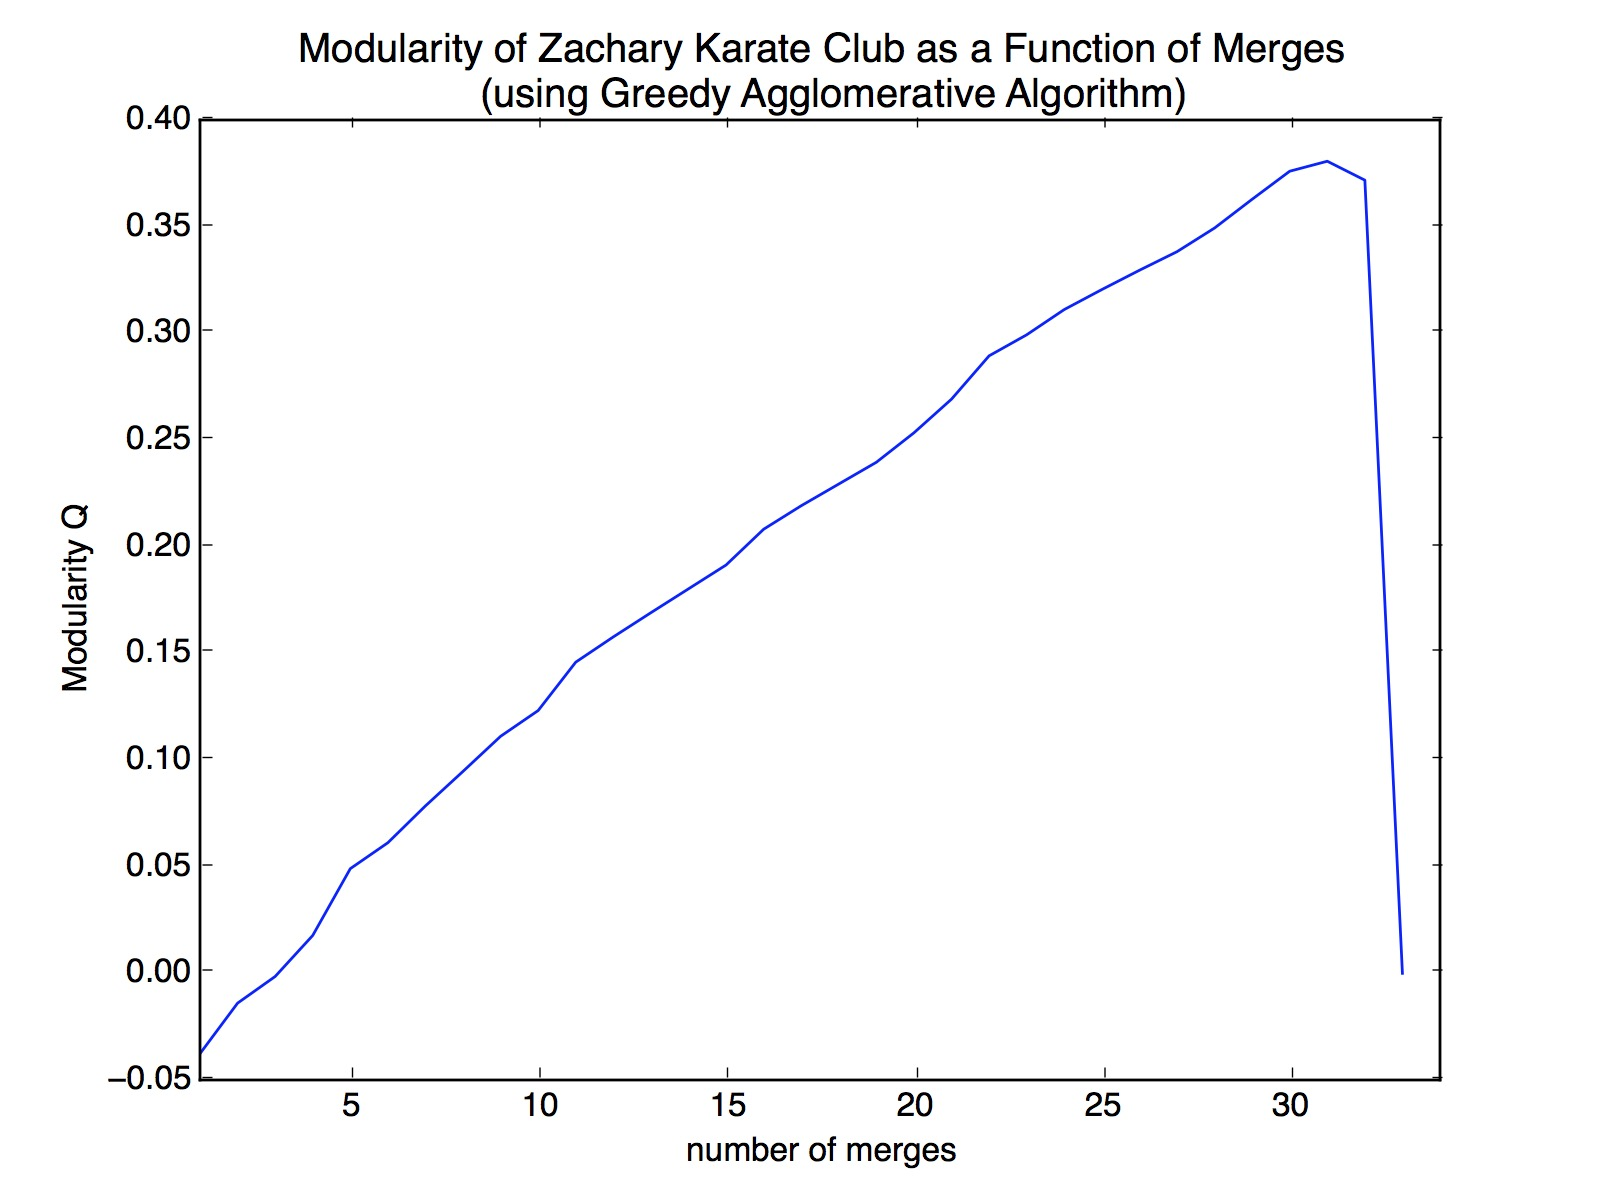
\includegraphics[scale=.15]{karateMerge.jpg}\\
The Normalized Mutual Information is $\frac{2I(C,C')}{H(C)+H(C')}$\\
where $H(C) = -\frac{17}{34} log_2 {\frac{17}{34}} - \frac{17}{34} log_2 {\frac{17}{34}}=1$\\
 $H(C') =   -\frac{8}{34} log_2 {\frac{8}{34}} - \frac{9}{34} log_2 {\frac{9}{34}} - \frac{17}{34}log_2{\frac{17}{34}} =     1.498751$\\
 and $I(C,C') = H(C) - H(C|C') =   1 - (\frac{8}{34} log_2 {1} -\frac{8}{34} log_2 {\frac{8}{9}} -\frac{1}{34} log_2 {\frac{1}{9}} -\frac{1}{34} log_2 {\frac{1}{17}} -\frac{16}{34} log_2 {\frac{16}{17}} )$\\
 \indent $=1.0-.0.294594 = 0.705406$\\
 $NMI = \frac{2(0.705406)}{2.498751} = 0.564607$\\\\
 Since NMI = 0.564607, this would suggest that, without knowing the 'truth on the ground',' it is possible to make relatively accurate, but not perfect, predictions about group membership with the greedy agglomerative algorithm.  It is interesting that the greedy algorithm gave three partitions, while the truth on the ground was made up of only two.  Nodes 2 and 3 seem to be the driving cause of this added cluster, forming many triangles with each other and surrounding nodes, with node 1 doing the same for the remaining nodes in the original (red) partition.\\
\\\\
4. Assortativity/modularity was calculated using the iGraph library for Python, as the modularity and assortativity functions therein are calculated using the same methods as presented in class and lecture notes.\\
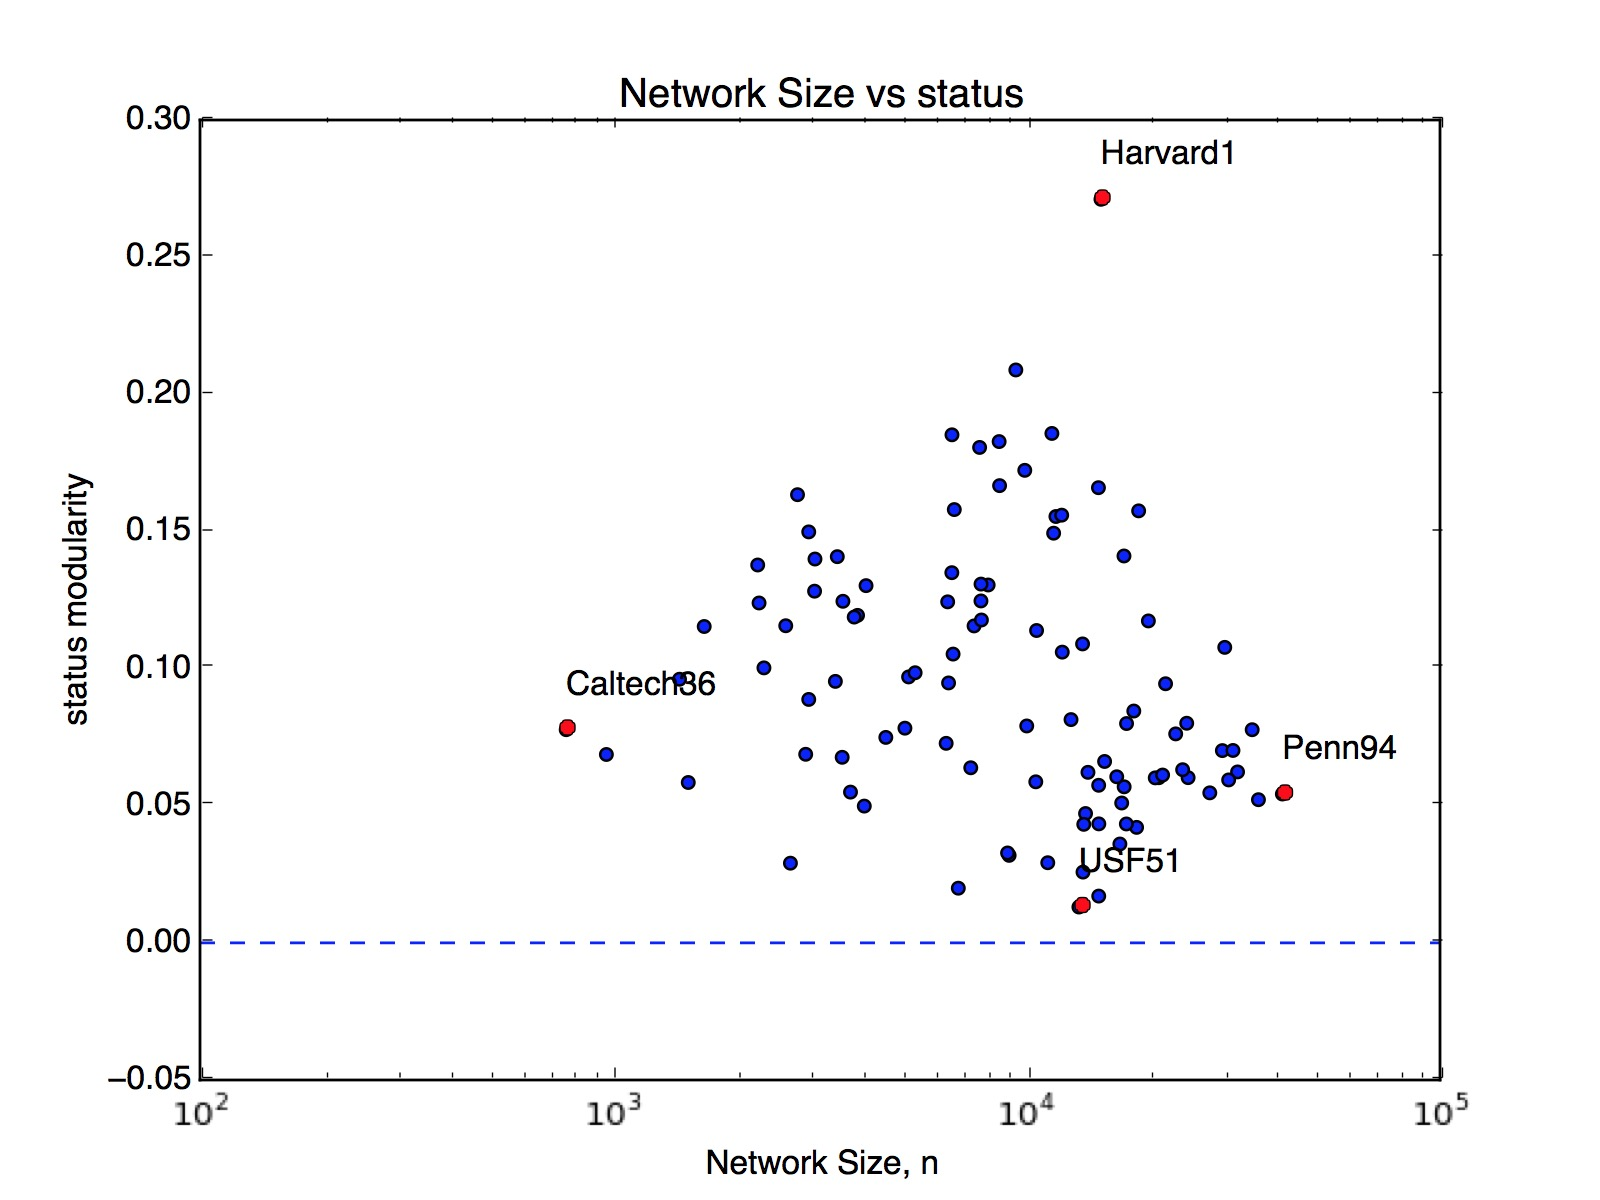
\includegraphics[scale=.15]{status.jpg}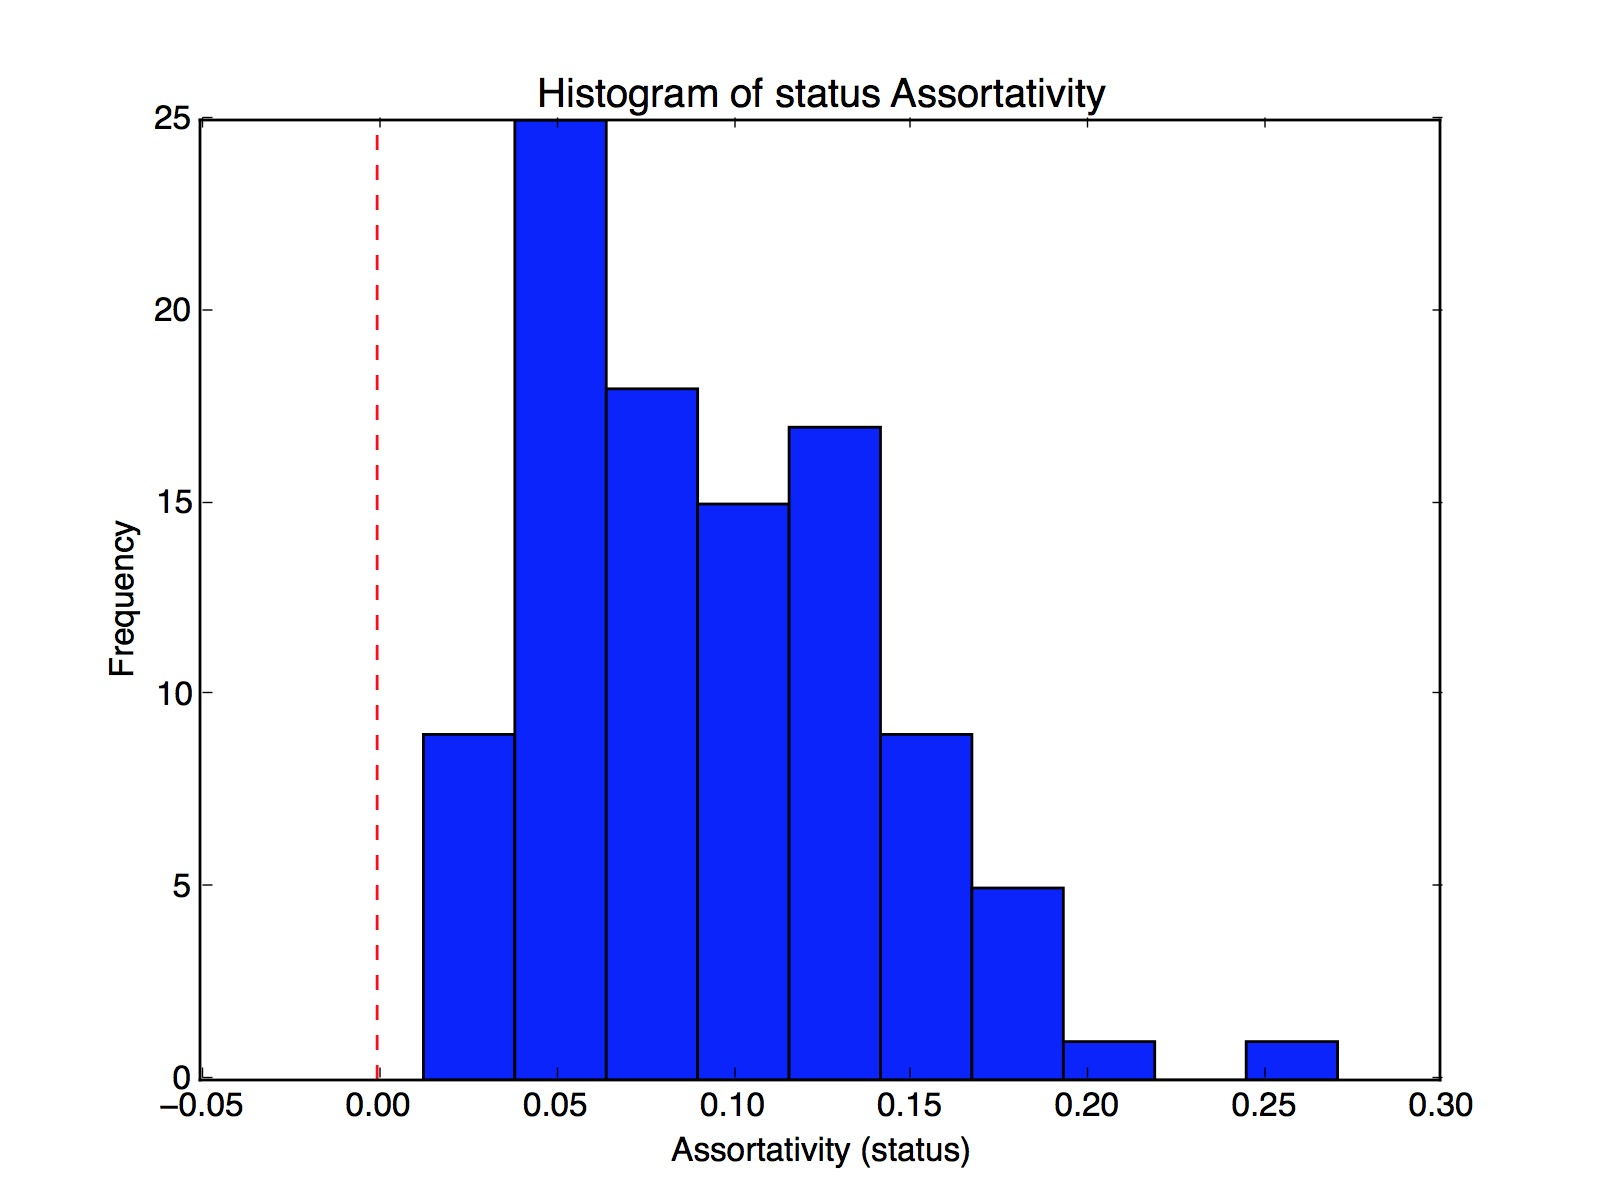
\includegraphics[scale=.15]{statusHist.jpg}\\
\indent Network size and modularity of status show distinct homophily.  Networks of all sizes exhibit positive modularity with respect to status (faculty, student, alumni, etc).  The most common degree of assortativity is around the 0.05 range, but the histogram has a rather long, positive tail.  This seems logical, since current students most likely connect with other students, faculty to faculty, etc.  Many universities most likely have a policy regarding faculty/student interactions outside of official business, so this may act to reinforce the homophily of the networks by actively discouraging connections between some groups.\\\\
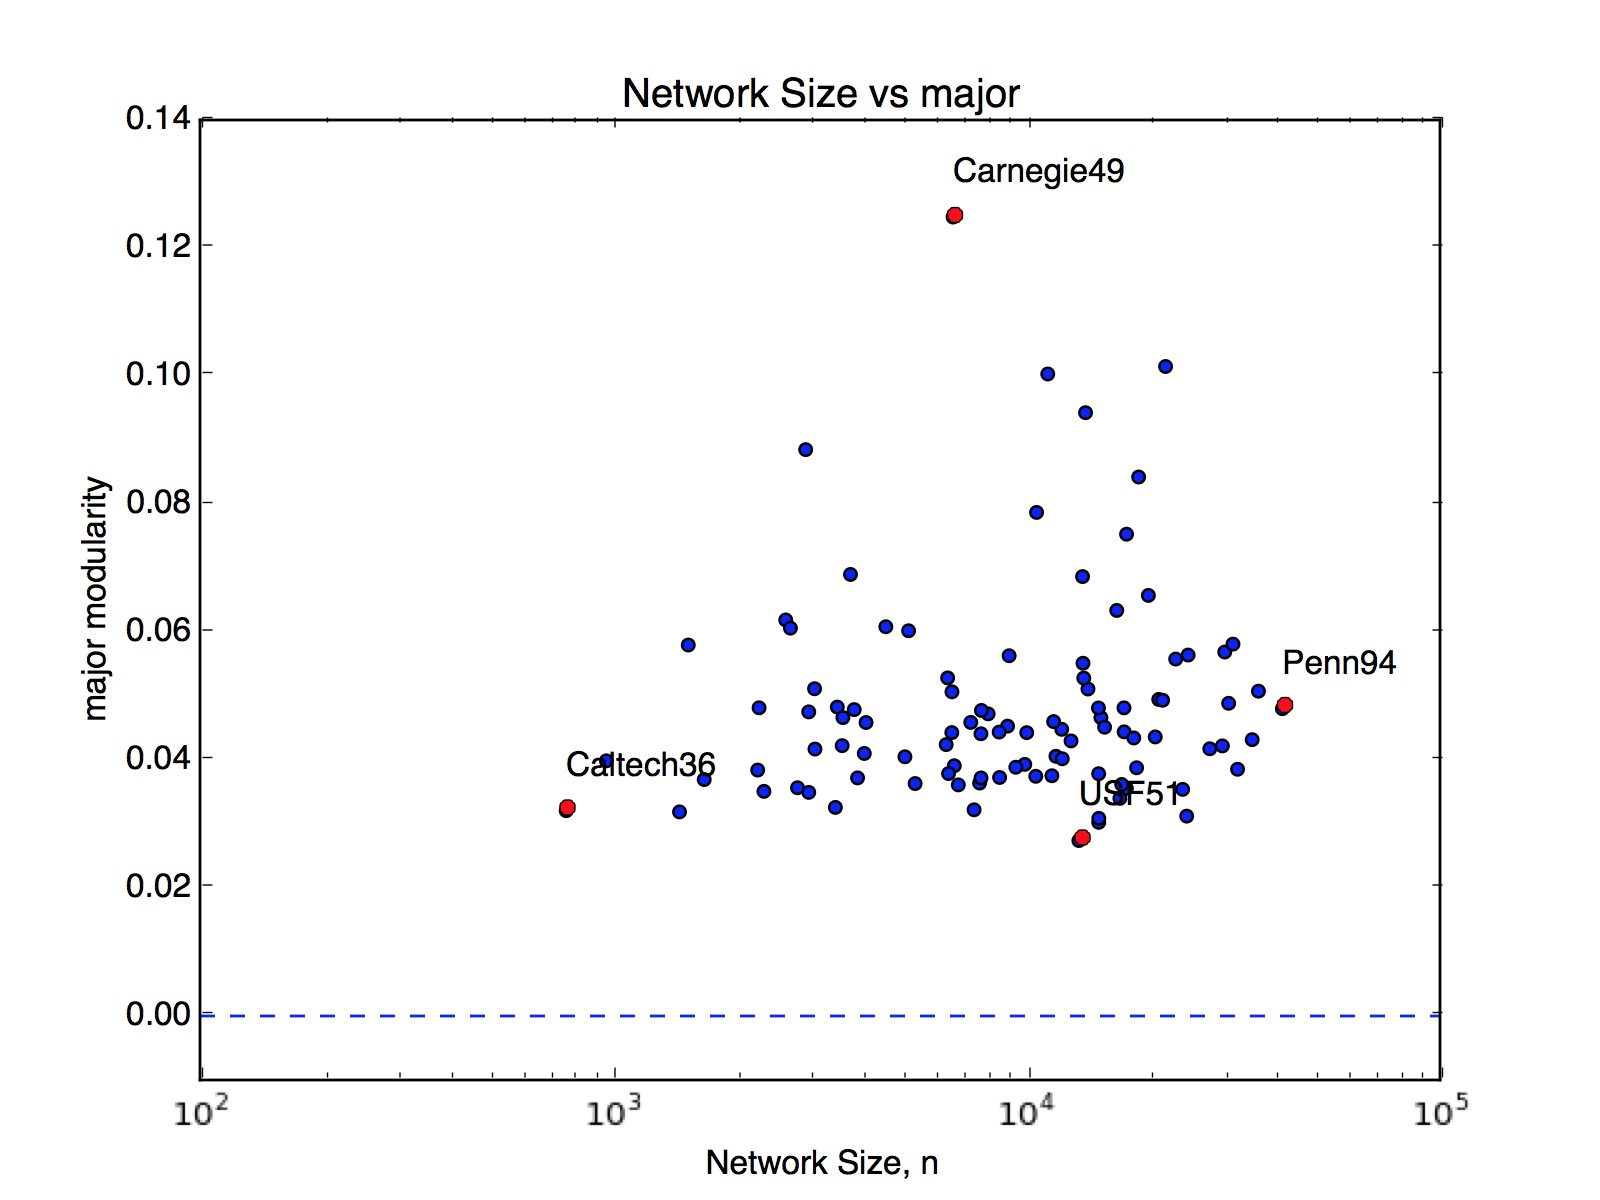
\includegraphics[scale=.15]{major.jpg}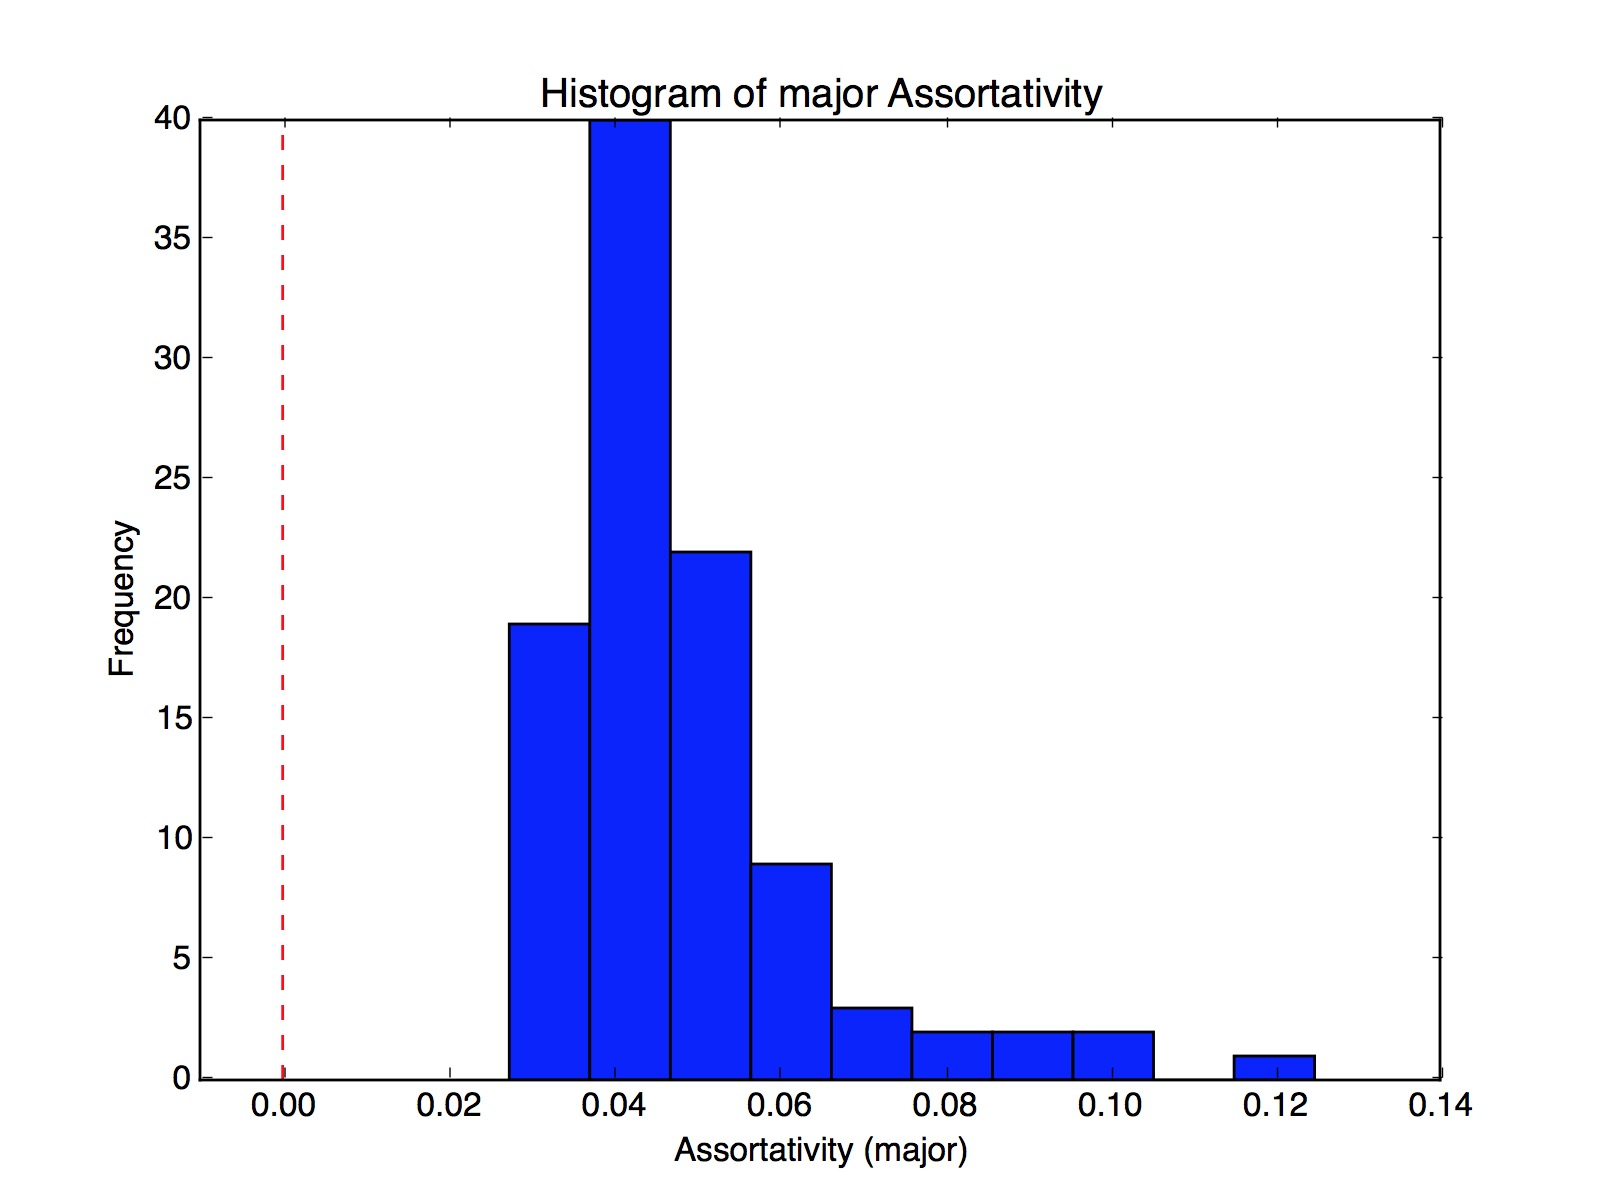
\includegraphics[scale=.15]{majorHist.jpg}\\
\indent Networks also exhibit homophily with regards to major.  The distribution is considerably more narrow than seen in the status data, with 40\% of networks having assortativity with respect to major at around 0.045.  Again, this is not surprising, considering that students most likely spend a lot of time with other students of the same major.  It is impossible to tell from the data given if these are purely 'friendship' connections, or if the data reflects a more academic connection between nodes, such as project or study groups.\\\\
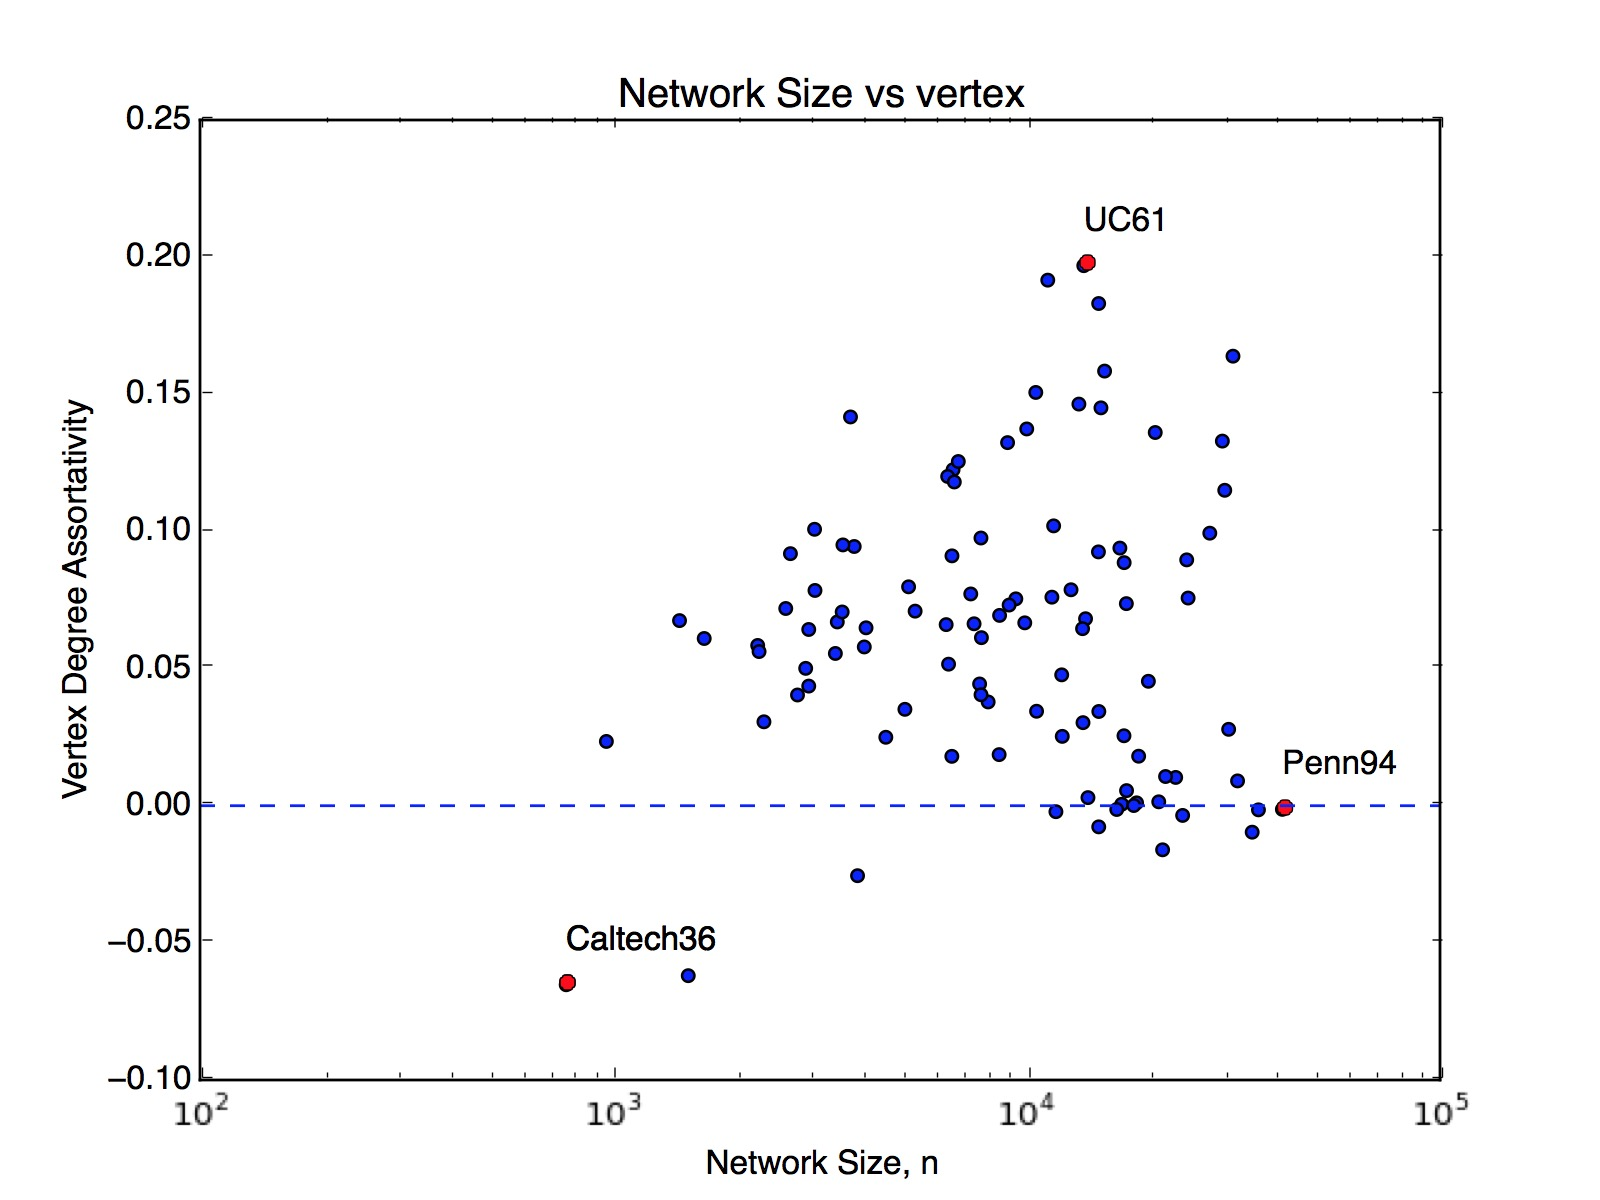
\includegraphics[scale=.15]{vertex.jpg}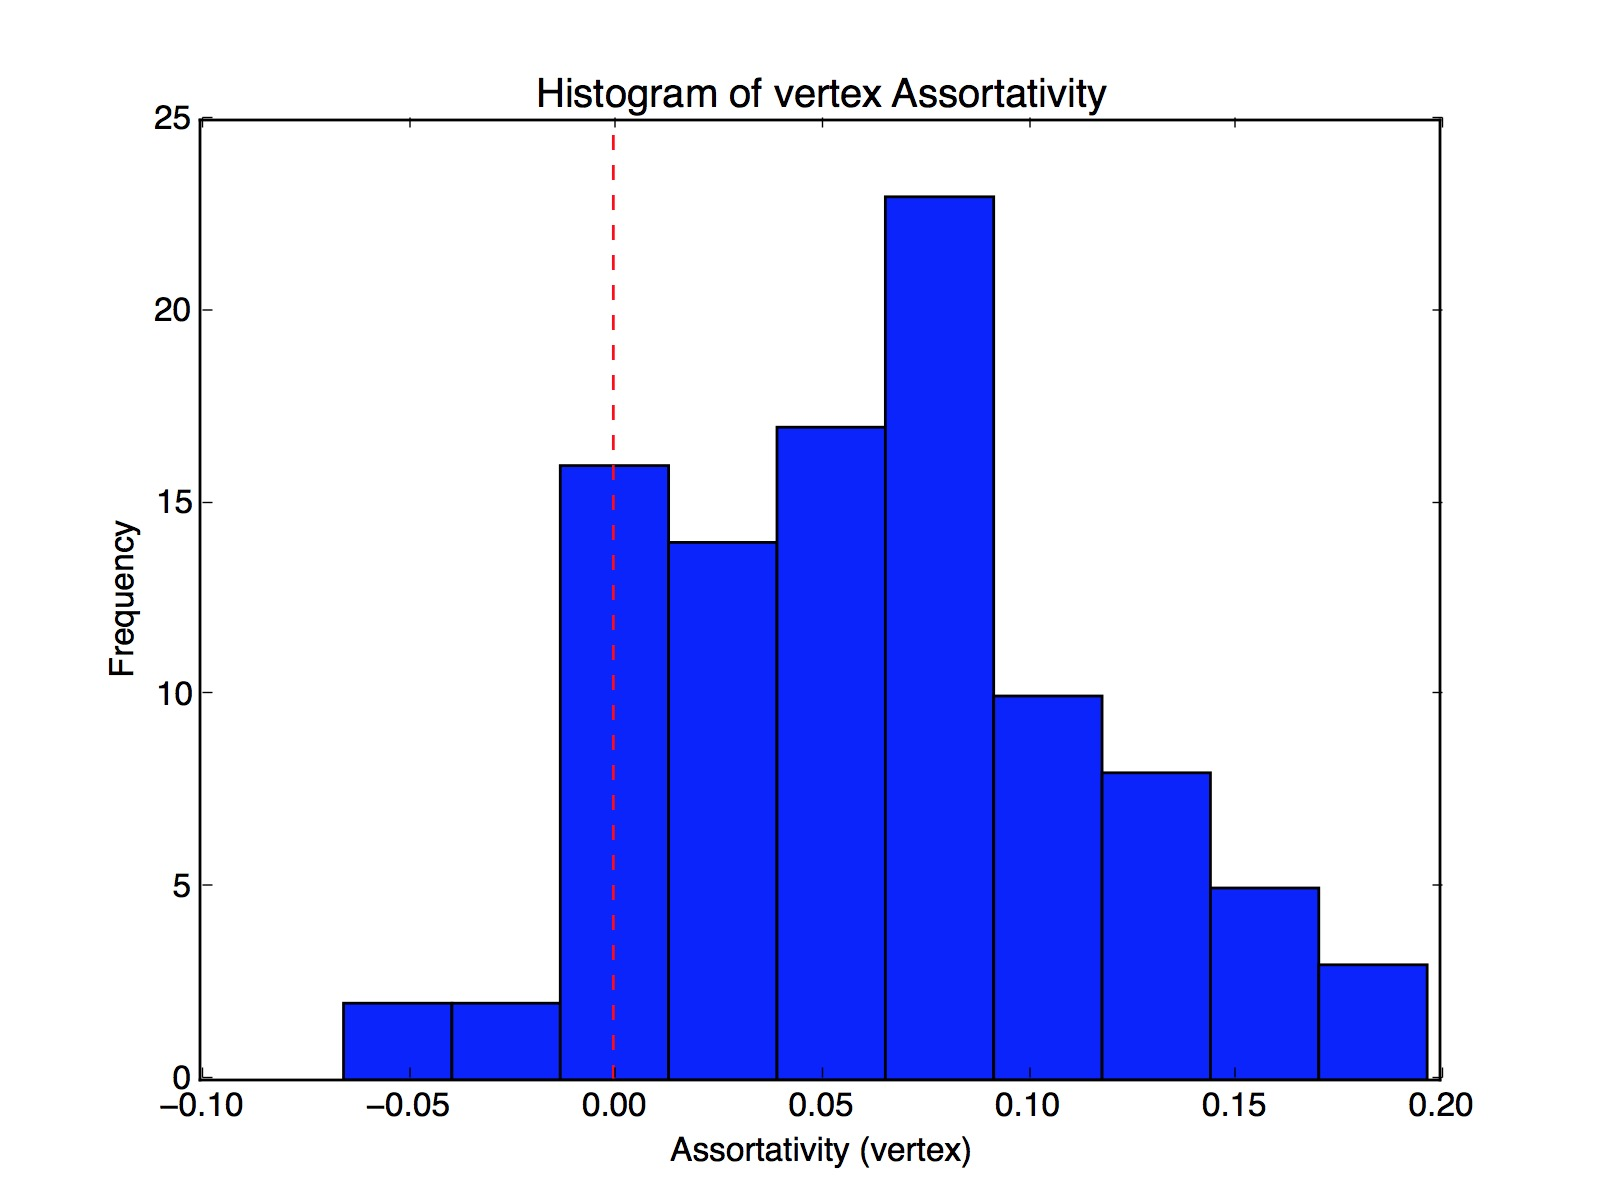
\includegraphics[scale=.15]{vertexHist.jpg}\\
\indent Assortativity with respect to vertex degree exhibits what seems to be the widest range of assortativity of all data sets examined, with some universities showing negative assortativity.  However, the histogram shows a wide distribution from 0.0 to 0.75, and with a long positive tail.  The lower vertex degree associations could be caused by the friendship paradox, as discussed earlier in class.  Since the average person's friends have more friends than she does, it follows that nodes link to nodes with a dissimilar degree number.  This does not explain the wide distribution, however.\\\\\\
6. To compute fractional sized of configuration model graphs, the networkx library for Python was used for convenience, as it has built-in functions for the generation of configuration model random graphs and finding the connected components therein.\\
\indent Part 1: To determine the mean fractional size of the largest component for a network with $n=10^4$ vertices, and with $p_1 = 0.6$ and $p_3 = 1-p_1$, 2663 iterations were performed.  Each iteration consisted of the generation of a random graph by the networkx.configuration\_model() function, using randomly generated degree sequences, matching the probabilities given.  The number 2663 was chosen to achieve a 99\% confidence level and a confidence interval of 2.5$^*$.  Under these conditions, the mean fractional size of the specified random network was 0.64204.\\
\indent Part 2:  Again using the networkx library, 666 iterations were performed for each $p_1$ value, from $p_1 = 0.01$ to $p_1 = 1.0$.  666 iterations were done to achieve a confidence level of 99\% and a confidence interval of 5$^*$, giving the following results:\\
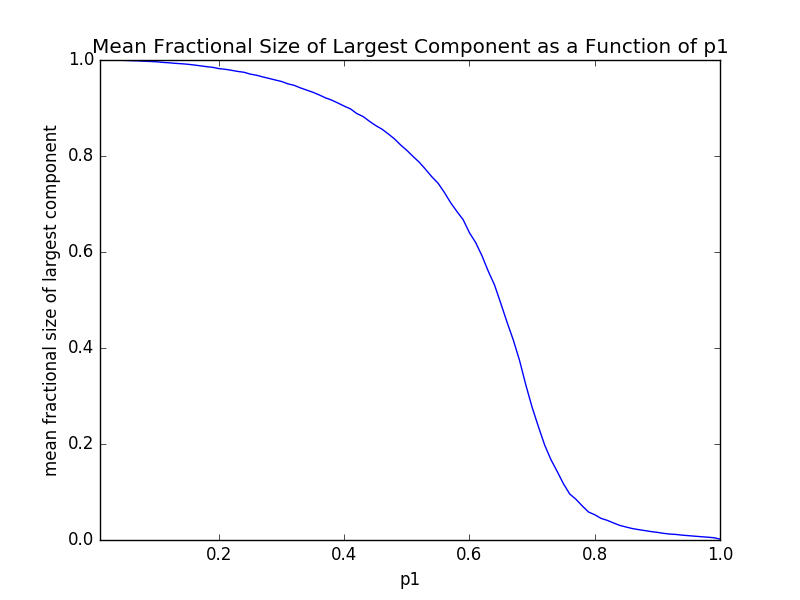
\includegraphics[scale=.5]{meanFractionalSize.png}\\
\indent The phase change, where the giant component disappears, happens as $p_1$ grows larger than 0.6 .\\\\\\
$^*$ per http://www.surveysystem.com/sscalc.htm\\\\\\\\\\\\\\
\inputminted[linenos,fontsize=\scriptsize]{python}{PS3.py}
\inputminted[linenos,fontsize=\scriptsize]{python}{Q42.py}
\inputminted[linenos,fontsize=\scriptsize]{python}{ec.py}
\inputminted[linenos,fontsize=\scriptsize]{python}{plotter.py}
\end{document}  